% The testflow support page is at:
% http://www.michaelshell.org/tex/testflow/



\documentclass[conference]{IEEEtran}

% *** CITATION PACKAGES ***
%
\usepackage{cite}

% *** GRAPHICS RELATED PACKAGES ***
%
\ifCLASSINFOpdf
 \usepackage[pdftex]{graphicx}
  % declare the path(s) where your graphic files are
  % \graphicspath{{../pdf/}{../jpeg/}}
  % and their extensions so you won't have to specify these with
  % every instance of \includegraphics
  % \DeclareGraphicsExtensions{.pdf,.jpeg,.png}
\else
  % or other class option (dvipsone, dvipdf, if not using dvips). graphicx
  % will default to the driver specified in the system graphics.cfg if no
  % driver is specified.
  % \usepackage[dvips]{graphicx}
  % declare the path(s) where your graphic files are
  % \graphicspath{{../eps/}}
  % and their extensions so you won't have to specify these with
  % every instance of \includegraphics
  % \DeclareGraphicsExtensions{.eps}
\fi

% *** MATH PACKAGES ***
%
\usepackage{mathtools}  
\usepackage{amsmath}
\usepackage{amssymb}
\usepackage{tabulary}
\usepackage{booktabs}
\DeclarePairedDelimiter\abs{\lvert}{\rvert}%
\DeclarePairedDelimiter\norm{\lVert}{\rVert}%

\interdisplaylinepenalty=2500

% *** SPECIALIZED LIST PACKAGES ***
%
\usepackage{algorithmic,algorithm}


% *** ALIGNMENT PACKAGES ***
%
%\usepackage{array}

% *** SUBFIGURE PACKAGES ***
%\ifCLASSOPTIONcompsoc
%  \usepackage[caption=false,font=normalsize,labelfont=sf,textfont=sf]{subfig}
%\else
%  \usepackage[caption=false,font=footnotesize]{subfig}
%\fi

% *** FLOAT PACKAGES ***
%
%\usepackage{fixltx2e}

%\usepackage{stfloats}

% *** PDF, URL AND HYPERLINK PACKAGES ***
%
\usepackage{url}

% correct bad hyphenation here
\hyphenation{op-tical net-works semi-conduc-tor}


\begin{document}
\title{Heterogeneous LDPC Decoder Algorithm on ARM and GPU of Mobile Devices}

% author names and affiliations
% use a multiple column layout for up to three different
% affiliations
\author{\IEEEauthorblockN{Roohollah Amiri}
\IEEEauthorblockA{Department of Electrical and\\Computer Engineering\\
Boise State University\\
Email: roohollahamiri@boisestate.edu}
\and
\IEEEauthorblockN{Hani Mehrpouyan}
\IEEEauthorblockA{Department of Electrical and\\Computer Engineering\\
Boise State University\\
Email: hanimehrpouyan@boisestate.edu}
}

% use for special paper notices
%\IEEEspecialpapernotice{(Invited Paper)}


% make the title area
\maketitle

% As a general rule, do not put math, special symbols or citations
% in the abstract
\begin{abstract}

Low density parity check (LDPC) codes have been extensively applied in mobile communication systems due to their excellent error correcting capabilities. However, their wide adoption has been hindered by the high complexity of the LDPC decoder. Although to date, dedicated hardware has been used to implement low latency LDPC decoders, recent advancements in the architecture of mobile processors has made it possible to develop software solutions. Here, unlike prior solutions that are based on either graphic processing units (GPUs) or advanced RISC machine (ARM) architectures, we propose a heterogeneous LDPC decoder that uses both the ARM and GPU processors of a mobile device to achieve efficient real-time decoding. The proposed solution is implemented on an NVIDIA development kit, where our results indicate that we can reduce the load on either the GPU or the ARM processor through the proposed heterogeneous structure, which in turn allows these resources to support other applications, simultaneously.

\end{abstract}

% no keywords

\IEEEpeerreviewmaketitle

\section{Introduction}
% no \IEEEPARstart
% LDPC , Usages, Complexity
Originally proposed by Robert Gallager in 1962 \cite{art_gallager} and rediscovered by MacKay and Neal in 1996 \cite{art_macKay} Low Density Parity Check (LDPC) codes have been adopted by a wide range of applications including many communication standards such as WiFi (IEEE 802.11n), 10 Gigabit Ethernet (IEEE 802.3an), Long Term Evolution (LTE) and DVB-S2. Recently, Chung and Richardson \cite{art_shannon} showed that a class of LDPC codes can approach the Shannon limit to within 0.0045 dB. However, the error correcting strength of these codes comes at the cost of very high decoding complexity \cite{art_ldpc_cpu1}. Moreover, to date, there are no closed-form solutions to determine the performance of LDPC codes in various wireless channels and systems. Thus, performance evaluation is typically carried out via simulations on computers or dedicated hardwares \cite{art_memory_coalesced}.

% Initial implementation
Since LDPC decoding algorithms are computationally-intensive and need powerful computer architecture to result in low latency and high throughput, to date, most LDPC decoders are implemented using application-specific integrated circuits (ASIC) or field-programmable gate array (FPGA) circuits \cite{art_ldpc_OpenCl_1}. However, their high speed often comes at a price of high developement cost, low programming flexibility \cite{art_convolutional} and it is very challenging to design decoder hardware that supports various standards and multiple data rates \cite{art_cuda_openmp}. On the other hand, iterative LDPC decoding schemes based on the sum-product algorithm (SPA) can fully be parallelized, leading to high-speed decoding \cite{art_shannon}. For these reasons, designers have recently focused on software implementations of LDPC decoders on multi/many-core devices \cite{art_massively} to meet the performance requirements of current communication systems through Software Defined Radio (SDR). As in terms of multi-core architectures, researchers have used CPUs \cite{art_cpu_gpu, art_ldpc_cpu0}, GPUs \cite{art_memory_coalesced, art_massively, art_optimize_0} and advanced RISC machine (ARM) \cite{art_ldpc_cpu0, art_neon} architectures to develop high throughput, low latency SDRs. 

%CPUs
In microarchitectures, increasing clock frequencies to obtain faster processing peorformance has reached the limits of silicon based architectures. Hence, to achieve gains in processing performance, other techniques based on parallel processing is being investigated \cite{art_ldpc_cpu1}. Todays' multi-core architectures support Single Instruction Multiple Data (SIMD), Single Programm Multiple Data (SPMD) and Single Instruction Multiple Threads (SIMT). The general purpose multi-core processors replicate a single core in a homogeneous way, typically with a x86 instruction set, and provide shared memory hardware mechanisms\cite{art_massively}. Such multi-core structures can be programmed at a high level by using different software technologies \cite{art_multicore_techs} such as OpenMP \cite{art_openMp_book} which provides an effective and relatively straightforward approach for programming general-purpose multi-cores. In \cite{art_cuda_openmp}, OpenMP is used to generate address patterns as a part of their LDPC decoder structure. On the other hand newer microarchitectures are trying to provide larger SIMD units for vector processing like Streaming SIMD Extensions (SSE), Advanced Vector Extensions (AVX) and AVX2 \cite{art_intel_sse} on Intel Architectures. In \cite{art_ldpc_cpu1}, the authors have used Intel SSE/AVX2 SIMD units to efficiently implement a high throughput LDPC decoder.

%GPUs
Mainly due to the demands for visualization technology in the gaming industry, the performance of graphics processing units (GPUs) has significantly improved over the last decade. With many cores driven by a considerable memory bandwidth, recent GPUs are targeted for solving computationally intensive algorithms in a multithreaded and highly parallel fashion. Hence, researchers in the high-performance computing field are applying GPUs to general-purpose applications (GPGPU). Pertaining to the field of communication, researchers have used Compute Unified Device Architecture (CUDA) from NVIDIA \cite{art_gpu_0,art_cuda_openmp, art_memory_coalesced, art_optimize_0, art_layered1} and Open Computing Language (OpenCL) \cite{art_ldpc_OpenCl} platforms to develop LDPC decoders on GPUs.

%ARMs and NEON
Due to large computing capacity of CPUs and GPUs, software based LDPC decoders have met the required throughputs of communication standards, although in wireless communication the end user's device is ususally a mobile device with an embedded system inside. Unlike today's powerful multi-core systems, embedded systems must operate on limited resources - small processors, tiny memory and low power. With an embedded system, it is about doing as much as you can with as little as you can. To solve this issue, ARM-based SDR systems have been proposed in recent years \cite{art_neon, art_ldpc_cpu0} with the goal of developing an SDR based LDPC decoder that provides high throughput and low latency on a low-power embedded system. The authors in \cite{art_neon} have used ARM processor's SIMD and SIMT programming models to implement an LDPC decoder that is based on parallel decoding of data frames. This approach allows reaching high throughput while maintaining low-latency. However, the proposed ARM based solution in \cite{art_neon}, is based on the assumption that the ARM processor is solely used for LDPC decoding but mobile devices need to support multiple applications simultaneously. Moreover, recent works in SDR LDPC embedded systems are missing the fact that today's mobile devices have powerful CUDA enabled GPUs which can play a significant role as a computing resource in an embedded system. This paper considers limited resources of a mobile device and proposes an algorithm to reach high throughput and low latency decoding on an embedded device.

%Contributions
The contributions of this paper are twofold. First, it proposes an LDPC decoder for an embedded device which exploits ARM SIMD units and GPU of the device together. This allows these resources to also support other applications on a mobile device. Second, as a consequence of this, by using the GPU of a mobile device, less memory from ARM processor is being used which is typically limited in an embedded system. The remainder of the paper is structured as follows. Section \ref{sec2} briefly introduces the LDPC code family and its decoding algorithms. Then the proposed heterogeneous algorithm on embedded targets is described in Section \ref{sec3}. Finally, \ref{sec4} gives experimental results and some comparisons with other ARM implementations.

\section{LDPC codes and their Decoding Processes}\label{sec2}

% LDPC Codes
LDPC codes are a class of linear block codes with a very sparse parity check matrix called H-matrix. Their main advantage is that they provide a performance which is very close to the channel capacity for a lot of different channels and linear time complex algorithms for decoding. Furthermore, they are suited for implementations that make heavy use of parallelism.

%representation
Basically there are two ways to represent LDPC codes. Like all linear block codes they can be described by their H-matrix, while they can be represented by a Tanner graph which is a bipartite graph. An LDPC graph consists of a set of variable nodes (VNs) , a set of check nodes (CNs), and a set of edges E. Each edge connects a variable node to a check node. For example, when the $(i,j)$ element of an H-matrix is '1', the $ith$ check node is connected to the $jth$ variable node of the equivalent Tanner graph. Figure \ref{tanner} illustrate the equivalent Tanner graph for $(10,5)$ LDPC code with H-matrix in \eqref{H-matrix}.

\begin{equation}\label{H-matrix}
H=
  \begin{bmatrix}
    1 & 1 & 1 & 1 & 0 &0 &0 &0 &0 &0 \\
    1 & 0 & 0 & 0 & 1 &1 &1 &0 &0 &0 \\
    0 & 1 & 0 & 0 & 1 &0 &0 &1 &1 &0 \\
    0 & 0 & 1 & 0 & 0 &1 &0 &1 &0 &1 \\
    0 & 0 & 0 & 1 & 0 &0 &1 &0 &1 &1 \\
  \end{bmatrix}
\end{equation}

\begin{figure}[h]\label{tanner}
\begin{centering}
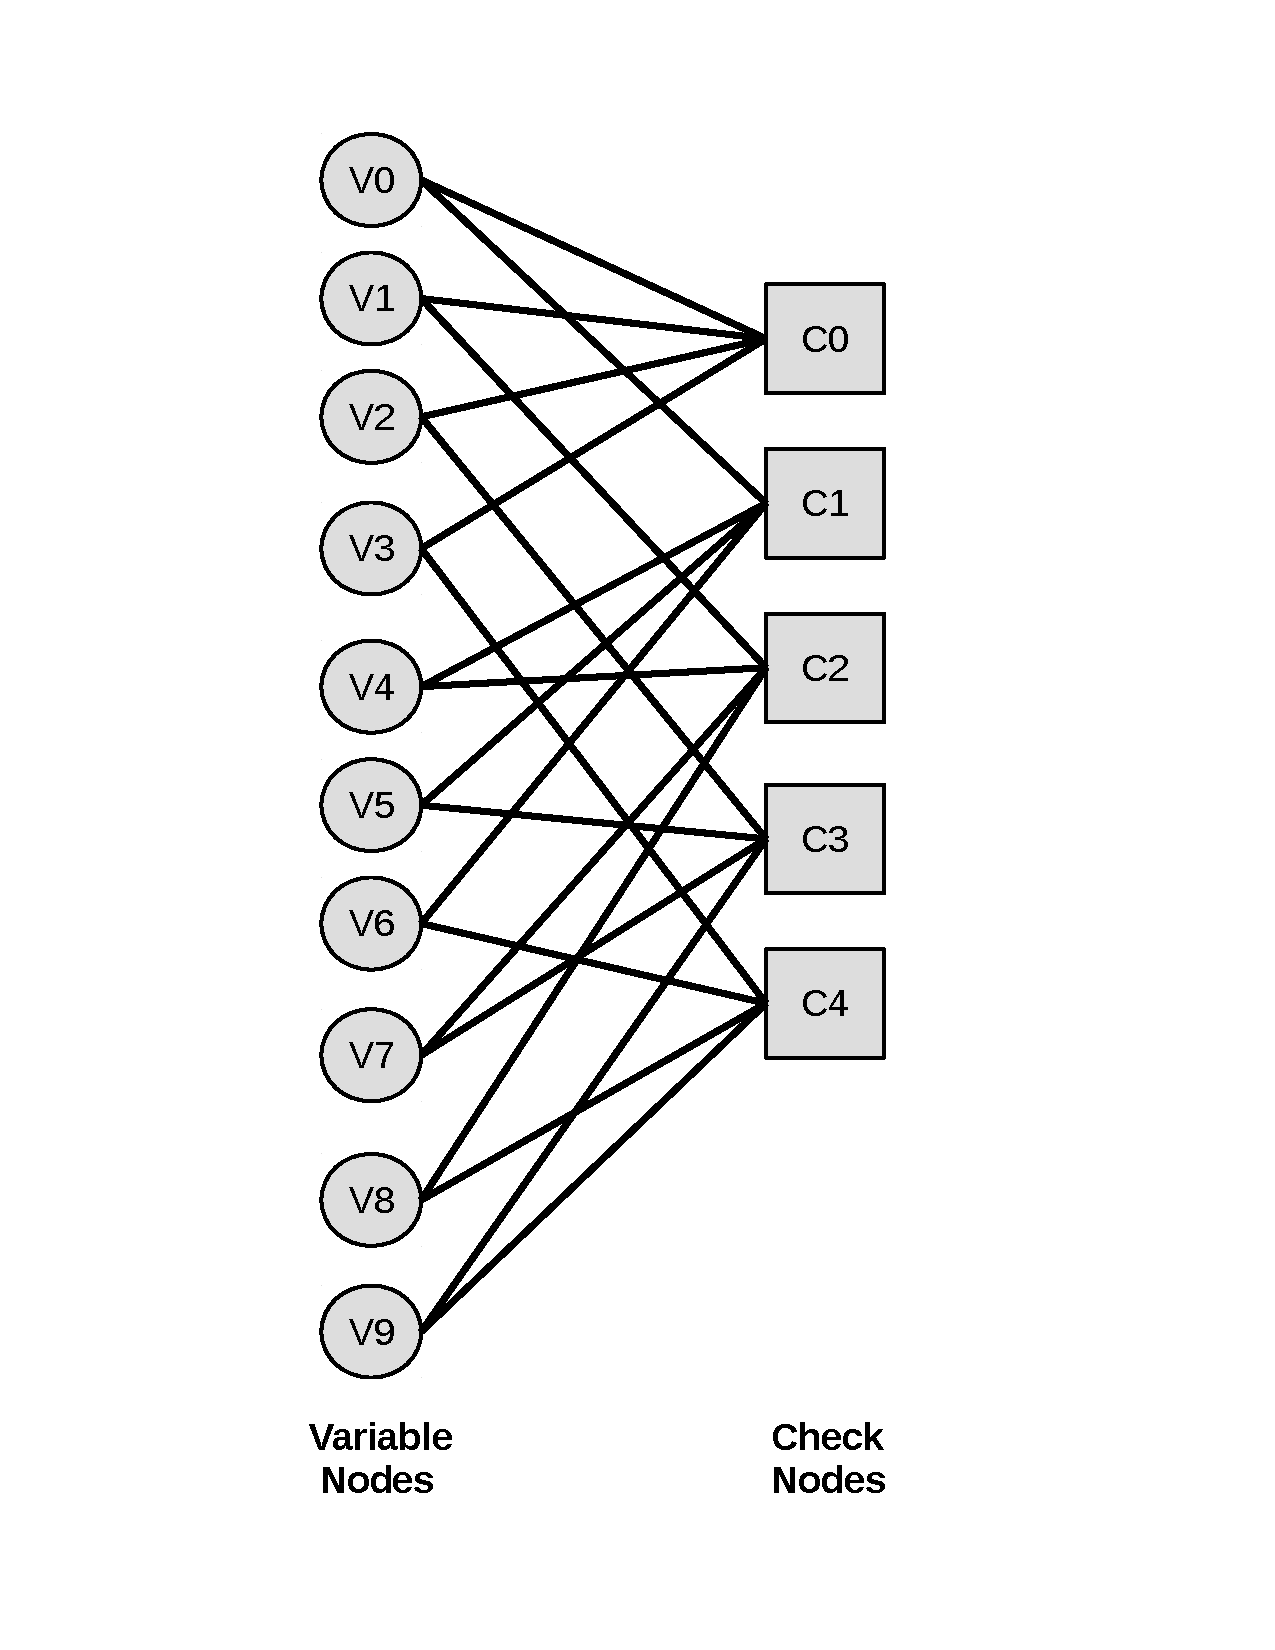
\includegraphics[scale=0.35]{tanner.pdf}
\caption[width=.3\textwidth]{An example of Tanner graph}
\end{centering}
\end{figure}

%Decoding
Many works as in \cite{art_massively, art_ldpc_cpu0,art_ldpc_OpenCl,art_gpu_0} focused on mapping LDPC decoders on multi-core architectures. Most of these works are based on the standard two-phase message passing (TPMP) schedule described in \cite{art_massively}. This algorithm works in two phases. In the first phase, all the variable nodes send messages to their neighboring parity check nodes, and in the second phase the parity check nodes send messages to their neighboring variable nodes. Due to transcendental operations and relying of message passing algorithm to the estimation of noise standard deviation, in practice Min-Sum (MS) variants are prefered by designers \cite{art_neon}. This algorithm is provided in Algorithm 1.

\begin{algorithm}\label{algorithm1}
\renewcommand\thealgorithm{}
\caption{Flooding Min-Sum algorithm}
\begin{algorithmic}[1]
\STATE \textbf{Kernel 1:} Initialization
\FORALL{$m \in C, n \in V$}
%\IF{$H_{mn}==1$}
\STATE
$Lq_{nm}=0$%LP_n=\dfrac{2y_n}{\sigma^2}.$
%\ENDIF
\ENDFOR
\FORALL{$t=1 \rightarrow (iter\_max)$}
\STATE \textbf{Kernel 2:} LLR of message $CN_m$ to $BN_n$
\FORALL{$m \in C, n \in V$}
\STATE $\alpha_{nm} \triangleq sign(Lq_{nm}),$
\STATE $\beta_{nm} \triangleq \abs{Lq_{nm}},$
\STATE $Lr_{mn} = \prod\limits_{n' \in N(m)\backslash n} \alpha_{n'm} \min\limits_{n' \in N(m)\backslash n} \beta_{n'm}.$
\ENDFOR
\STATE \textbf{Kernel 3:} LLR of message $BN_n$ to $CN_m$
\FORALL{$m \in C, n \in V$}
\STATE $Lq_{nm} = LP_n + \sum\limits_{m' \in M(n)\backslash m} Lr_{m'n}.$
\ENDFOR  
\ENDFOR % End of Iter
\STATE \textbf{Kernel 4:} Hard decision from soft-values
\FORALL{$n \in V$}
\STATE $LQ_{n} = LP_n + \sum\limits_{m' \in M(n)} Lr_{m'n},$
\STATE $\forall n, \hat{c}=[LQ_n]>0.$
\ENDFOR
\end{algorithmic}
\addtocounter{algorithm}{-1}
\end{algorithm}

More efficient layered schedules, such as horizontal layered-based decoding algorithm, allow updated imformation to be utilized more quickly in the algorithm, thus, speeding up the decoding\cite{art_layered0, art_layered1}. In fact, the H-matrix can be viewed as a layered graph that is decoded sequentially. The work in \cite{art_gpu_0} has applied a form of layered belief propagation to irregular LDPC codes to reach 2x faster convergence in a given error rate. By using this method they have reduced memory bits usage by 45-50\%. The layered decoding (Algorithm 2) can be summarized as follow: all values for the check node computations are computed using variable node massages linked to them. Once, a check node is calculated, the corresponding variable nodes are updated immediately after receiving massages. This process is repeated to the maximum number of iterations.
\begin{algorithm}\label{algorithm2}
\renewcommand\thealgorithm{}
\caption{Horizontal Layered Min-Sum algorithm}
\begin{algorithmic}
\STATE \textbf{Kernel 1:} Initialization
\FORALL{$m \in C, n \in V$}
\STATE
$Lr_{mn}=0$
\ENDFOR
\FORALL{$t=1 \rightarrow (iter\_max)$}
\STATE \textbf{Kernel 2:} Process each CN one after another
\FORALL{$m \in C$}
\FORALL{$n \in V$}
\STATE $\alpha_{nm} \triangleq sign(Lq_{nm}),$
\STATE $\beta_{nm} \triangleq \abs{Lq_{nm}},$
\STATE $Lr'_{mn} = \prod\limits_{n' \in N(m)\backslash n} \alpha_{n'm} \min\limits_{n' \in N(m)\backslash n} \beta_{n'm}.$ \STATE\COMMENT{$Lr'_{mn}$ is the new calculated massage to $BN_n$}
\ENDFOR
\ENDFOR
\FORALL{$n \in V$}
\STATE $LQ'_n=LQ_n-Lr_{mn}+Lr'_{mn}$
\ENDFOR
\ENDFOR % END Iteration
\STATE \textbf{Kernel 4:} Hard decision from soft-values
\FORALL{$n \in V$}
\STATE $\forall n, \hat{c}=[LQ_n]>0.$
\ENDFOR
\end{algorithmic}
\addtocounter{algorithm}{-1}
\end{algorithm}

In algorithm 1, TPMP, the kernels 2 and 3 are updated by seperate processing and passed to each other iteratively. It means that variable nodes update, will not start until all check nodes are updated. Consdering that, algorithm 2, horizontal layered decoding, is composed of a single loop kernel with some data dependencies between consecutive loop iterations and in each iteration, the horizontal layers are processed sequentially from the top to the bottom layer \cite{art_quasi}.

Although layered algorithm is composed of a single loop kernel composed to two sequential kernels in standard algorithms, it has an irregular memory access as a major limitation. To solve this irregular memory access, a data interleaving/deinterleaving process is used before and after the decoding process in \cite{art_gpu_0, art_neon}, which is used in the proposing algorithm too. In \cite{art_gpu_0}, the GPU decoder achieves high throughputs but its latency that goes beyond seconds makes it suitable for simulation purposes only. On the other hand, the ARM decoder proposed in \cite{art_neon} uses all computing resources (4 existing cores) for LDPC decoding and does not take advantage of GPU processing on mobile devices. This paper uses one single core of ARM and the GPU device of a mobile processor to implement a high throughput and low latency LDPC decoder. By using one core of the ARM processor, there will be processing power for other applications of a mobile device and less memory of ARM processor will be used for decoding. On the other hand, since the GPU and ARM of a mobile device are sitting on a same die, the latency issues in \cite{art_gpu_0} are improved.

\section{Algorithm Mapping}\label{sec3}

An efficient implementation of the layered decoding algorithm is a challenging task. The drawbacks of this algorithm as in terms of programming are: (i) the number of computations respect to number of memory access is low; (ii) the data reusing between consecutive computations is low; (iii) it requires a large set of irregular memory access due to H-matrix structure \cite{art_ldpc_cpu1}. Considering these, a software-based decoder should take advantage of different parallelism levels offered by the target architecture to achieve high throughput efficiency. In this section, first the target architecture's features are presented. Then the decoding algorithm is detailed.

\subsection{Target architecture} \label{target_architecture}
In this study, we focused on embedded devices equipped with ARM and GPU processors. One example is Jetson K1 SoCs which contains a 4-core Cortex-A15 and a GPU processor.

ARM Cortex-A15 processor is composed of 15 integer/17-25 floating point pipeline stages. To limit the level of memory access latency, it has multi-level caches as 32 KB data + 32 KB instruction L1 cache per core and an integrated low-latency L2 cache controller, up to 4 MB per cluster. Each core includes a NEON SIMD unit which can execute up to 16 computations on 8-bit data simultaneously. As in terms of GU features, concurrent kernel execution capability of this device is most used in the proposed mapping. To achieve high throughput performance on such a low-power embedded processors, SIMD and SIMT programming models are exploited in the proposed LDPC decoder. In the next subsections, we detailed the different parallelism levels along with the implementation choices.

\subsection{Parallelism levels in the proposed algorithm}
To achieve high throughput performance, a software LDPC decoder has to exploit computation parallelism for taking advantage of multi-core architectures. Different parallelism levels are present in a layered decoding algorithm. \textbf{First parallelism level} is located inside the CN computations (Algorithm 2, loops located at line 8 and 15). It is possible to execute such computations in parallel, however this atomic parallelism level is hard to exploit due to the low complexity of computations. \textbf{Second parallelism level} is located at CN level (Algorithm 2, line 7). Two CN computations can be done in parallel if there is no data dependency. Thus this level is hard to exploit and inefficient. \textbf{Third parallelism level} is located at frame level (Complete Algorithm 2). A same computation sequence is executed over consecutive frames. This approach provides an efficient parallel processing algorithm. So we have used single instruction multiple data (SIMD) programming model to decode F frames in parallel. 

\subsection{Data Interleaving/deinterleaving}
The implementation of the parallel frame processing is subject to massive irregular memory access due to the structure of H-matrix. As a matter of fact, to process the same $VN_i$ element of the F frames at the same time, non-contiguous memory access would affect performance. To solve this issue, a data interleaving process has to be performed before and after decoding stage. So channel information coming from F frames are reordered to achieve an aligned memory data structure. This reordering is shown in Figure \ref{fig_intreleave}.

\begin{figure}[h]
\begin{centering}
\scalebox{0.25}{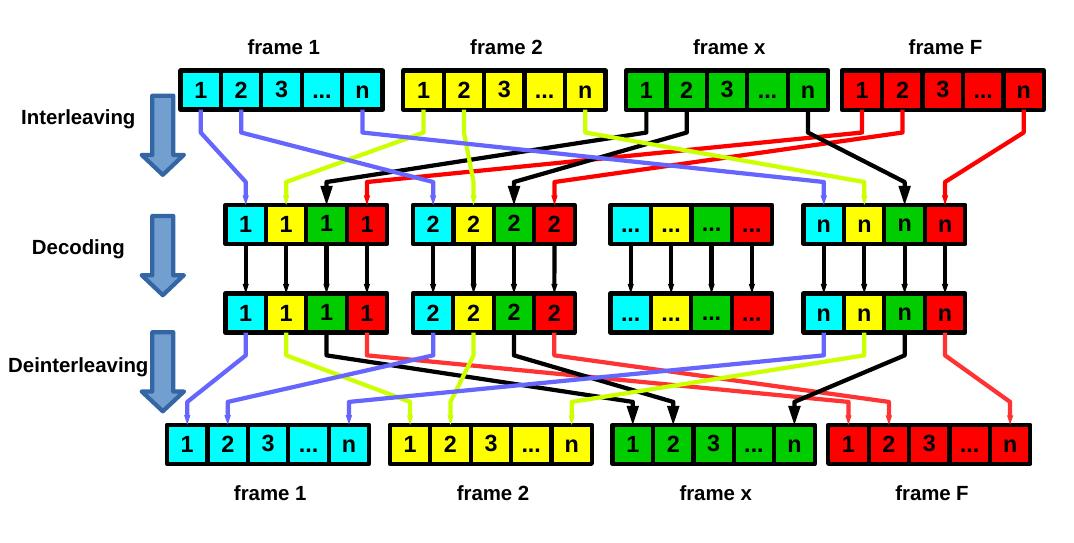
\includegraphics{inter1.jpg}}
\caption[width=.3\textwidth]{Data interleaving/deinterleaving process}
\label{fig_intreleave}
\end{centering}
\end{figure}

\subsection{Stream based parallelism}

SIMT programming model is used to decode W sets of F frames concurrently, with W the number of concurrent streams on the GPU device. This multi-core programming is specified by CUDA API. Each gpu stream is controlled by a \textit{pthread} called \textit{worker} on the host machine (which is an ARM in this case). Each \textit{worker} is responsible for its own sets of frames. By using stream based processing, the system can decode W$*$F frames at the same time. The whole LDPC decoder system model is shown in Figure \ref{fig_total}.

\begin{figure}[h]
\begin{centering}
\scalebox{0.5}{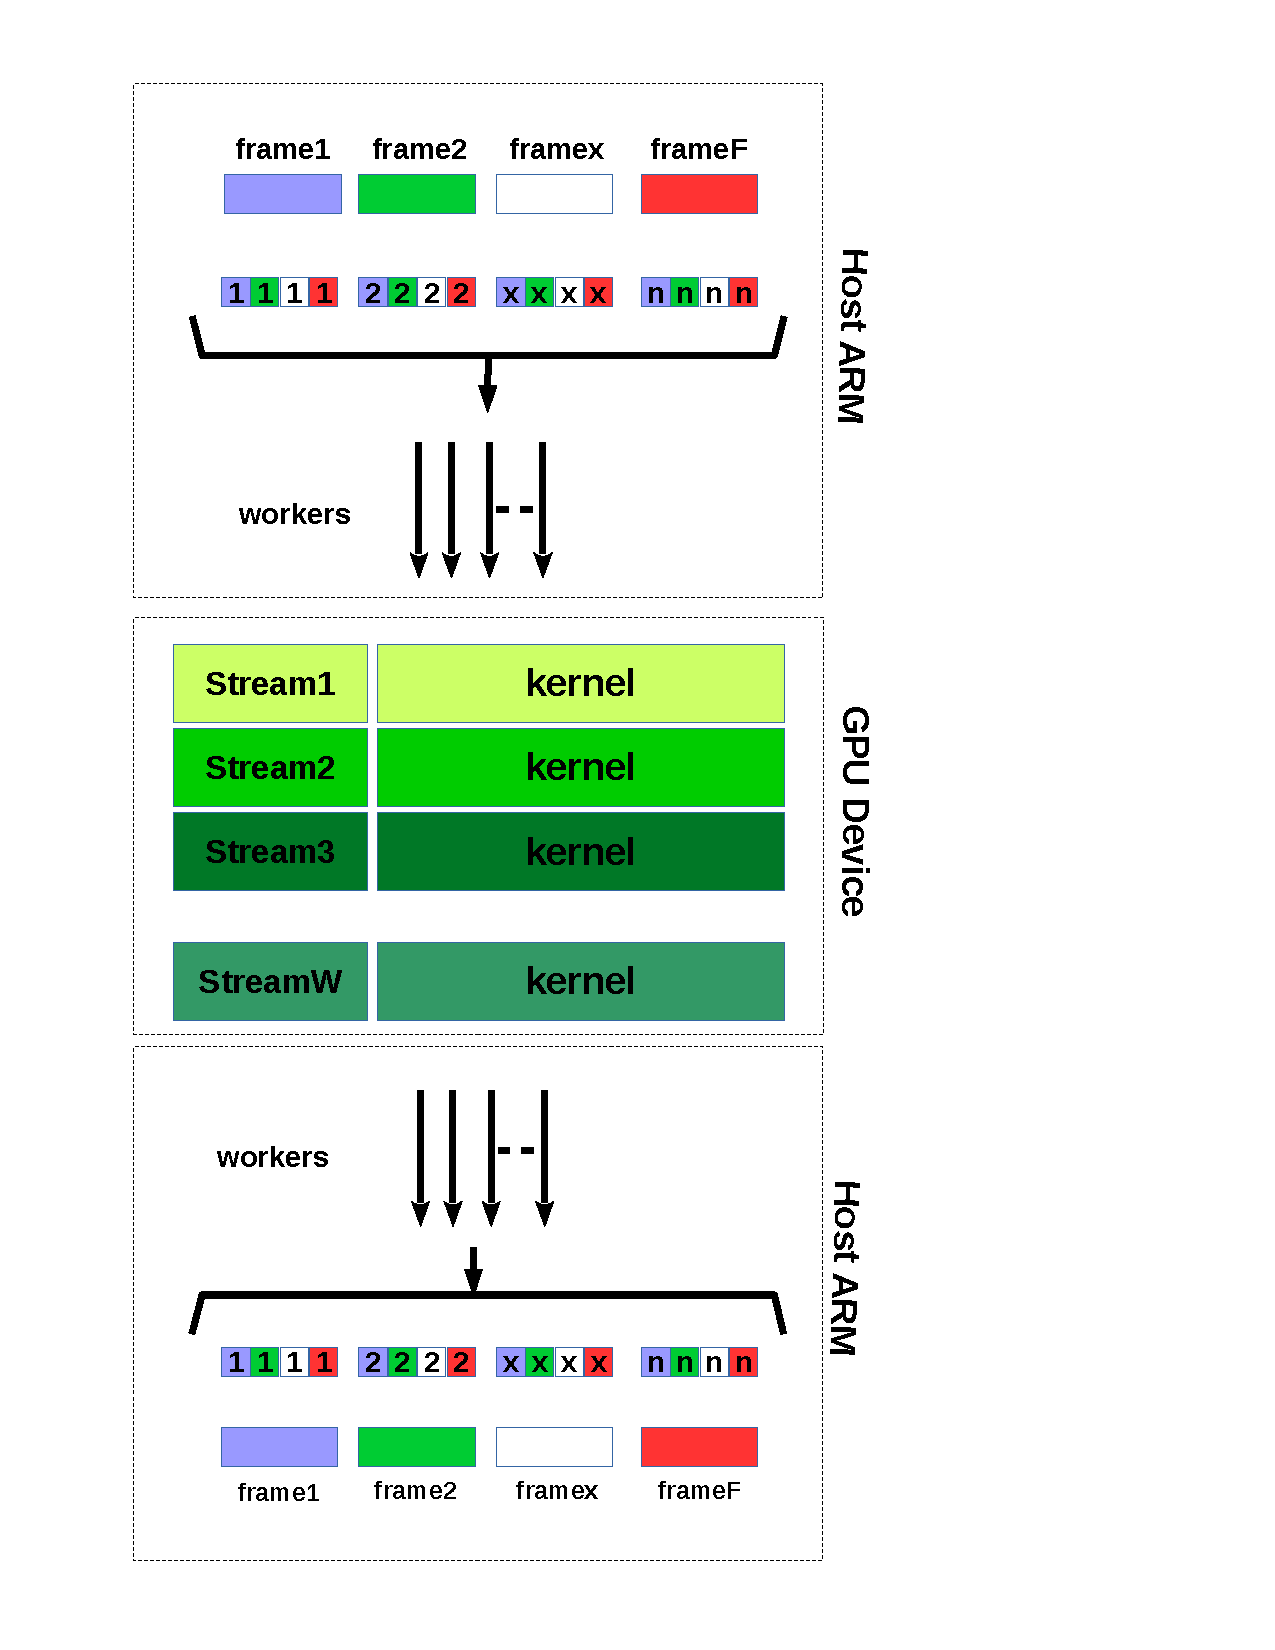
\includegraphics{total.pdf}}
\caption[width=.3\textwidth]{LDCP Decoder Data Flow}
\label{fig_total}
\end{centering}
\end{figure}

\section{Experimental Results} \label{sec4}

The experiments were carried out by decoding LDPC codes using NVIDIA Tegra K1 Socs. The programs compiled with GCC-4.8 and CUDA 6.5. The TK1 is composed of 4 cortex-A15 ARM processors and one NVIDIA Kepler "GK20a" GPU with 192 SM3.2 CUDA cores. The host platform uses a GNU/Linux kernel 3.10.40.

\subsection{Performance evaluation of heterogeneous algorithm} 


\subsection{Performance comparison with related works}


\section{Conclusion}
The conclusion goes here.

\newpage

\bibliographystyle{IEEEtran}
\bibliography{IEEEabrv,ldpcGpuTegra_bibliography}



% that's all folks
\end{document}


